\chapter{Streams}

% support for streaming
% recent data is valuable, long not so much
% queries are know, data is not

% receives unending/infinite data, runs static query
% memory is limited

% timestamps carry meaning (often implicit), can be approximate
% could not be monotonic?

% Results are approximate (with some guarantees) 

% Scheduling not up to system (recieves input)
% Order important
% State bounded, input unbounded

\section{Push Operators}
Data sources push into operators.

\subsection{Naive Implementation}
% code for operators


\subsection{PushBack}
% time
% resource usage
% multiple threads

\section{Time}
Systems often implicitly provide timestamps for pushed data, for example when joining data based on timestamps.
\begin{itemize}
    \item Needs to be consistent (same stream results in the same output data).
    \item Needs to be performant/low overhead (reduce backpressure).
\end{itemize}

\begin{definitionbox}{Processing-Time}
    Each operator timestamps data when it is pushed to the operator.
    \begin{minted}{cpp}
class SomeOperator : public Operator {
    // ... internal state
public:
    void process(InputRow data) override {
        auto data_timestamp = std::chrono::system_clock::now();
        // ... use data & data_timestamp
    }
};
    \end{minted}
    \begin{center}
        \begin{tabular}{c | c | c}
            \textcolor{red}{inconsistent} & \textcolor{red}{unpredicatable} & \textcolor{ForestGreen}{low-overhead} \\
        \end{tabular}
    \end{center}
\end{definitionbox}

\begin{definitionbox}{Ingestion-Time}
    Timestamp when received by the system (i.e the source object that pushes to the first operator).
    \begin{minted}{cpp}
class NetworkSource : public Source {
    // ... internal state
public:
    void run() override {
        for (;;) if (!network.buffer_empty()) {
            auto data_timestamp = std::chrono::system_clock::now();
            auto data = network.pop_next();
            // ... use data & data_timestamp
        }
    }
};
    \end{minted}
    \begin{center}
        \begin{tabular}{c | c | c}
            \textcolor{ForestGreen}{consistent} & \textcolor{red}{unpredicatable} & \textcolor{orange}{medium-overhead} \\
        \end{tabular}
    \end{center}
\end{definitionbox}
\begin{definitionbox}{Event-Time}
    Timestamps externally provided by the source supplying events to the data processing system as part of data input.
    \begin{itemize}
        \item System needs to ensure timestamps are ordered (external provider may not be correct). 
    \end{itemize}
    \begin{minted}{cpp}
class NetworkSource : public Source {
    // ... internal state
public:
    void run() override {
        for (;;) if (!network.buffer_empty()) {
            auto data = network.pop_next();
            // can just treat timestamp as normal data, or extract specially
            auto data_timestamp = data.timestamp;
            // ... use data & data_timestamp
        }
    }
};
    \end{minted}
    \begin{center}
        \begin{tabular}{c | c | c}
            \textcolor{ForestGreen}{consistent} & \textcolor{ForestGreen}{predicatable} & \textcolor{red}{high-overhead} \\
        \end{tabular}
    \end{center}
\end{definitionbox}

\subsection{In-Order Processing}
\begin{definitionbox}{In-Order Processing}
    Events are assumed to be entered in timestamp order (or by some other monotonically progressing attribute - e.g counter).
    \begin{itemize}
        \item Greatly simplifies stream system implementation, a powerful guarantee. 
        \item Difficult to ensure order guarantee holds (on a distributed, asynchronous system there is not global clock)
    \end{itemize}
\end{definitionbox}
While it is usually prohibitively difficult to implement In-Order processing, we still need to have some guarantees on ordering for queries that rely on in-order data.
\begin{itemize}
    \item If a single server is used to apply timestamps it can become a bottleneck.
    \item We can make some assumptions on bounds of how out-of-order messages can be received.
    \item We can reduce the \textit{In-Order} to a \textit{Sort-Order}.
\end{itemize}

\subsubsection{Transactions}
The stream of events is treated as a sequence of transactions.
\begin{itemize}
    \item All events are inserted into persistent database
\end{itemize}
\begin{minted}{sql}
-- Store all inputs to persistent backing table
ON IncomingEvent newEvent INSERT INTO event_backing_table VALUES (newEvent)

-- Stream out data (e.g by selecting based on a predicate)
SELECT * FROM event_backing_table WHERE some_predicate(x, y, newEvent);
\end{minted}
\begin{tabbox}{consbox}
    \textbf{Finite Memory} & Streams are infinite, persistent database must have older entries cleared/garbage collected. \\
\end{tabbox}

\subsubsection{Lateness Bounds}
A lateness bound is assumed for any event, events outside this bound are dropped.
\begin{minted}{sql}
ON IncomingEvent newEvent INSERT INTO event_backing_table VALUES (newEvent)
SELECT * FROM event_backing_table WHERE some_predicate(x, y, newEvent);

-- Delete old data from the table using the new event's timestamp
DELETE FROM event_a_backing_table WHERE timestamp < (newEvent.timestamp - LATENESS_BOUND);
\end{minted}
\begin{tabbox}[.7\textwidth]{consbox}
    \textbf{Tune Lateness Bound} & If the bound is too small (many tuples dropped), too large and memory resource becomes pressured by large backing table \\
\end{tabbox}

\subsubsection{Watermarks/Punctuation}
\unfinished

\subsection{Windows}
\begin{center}
    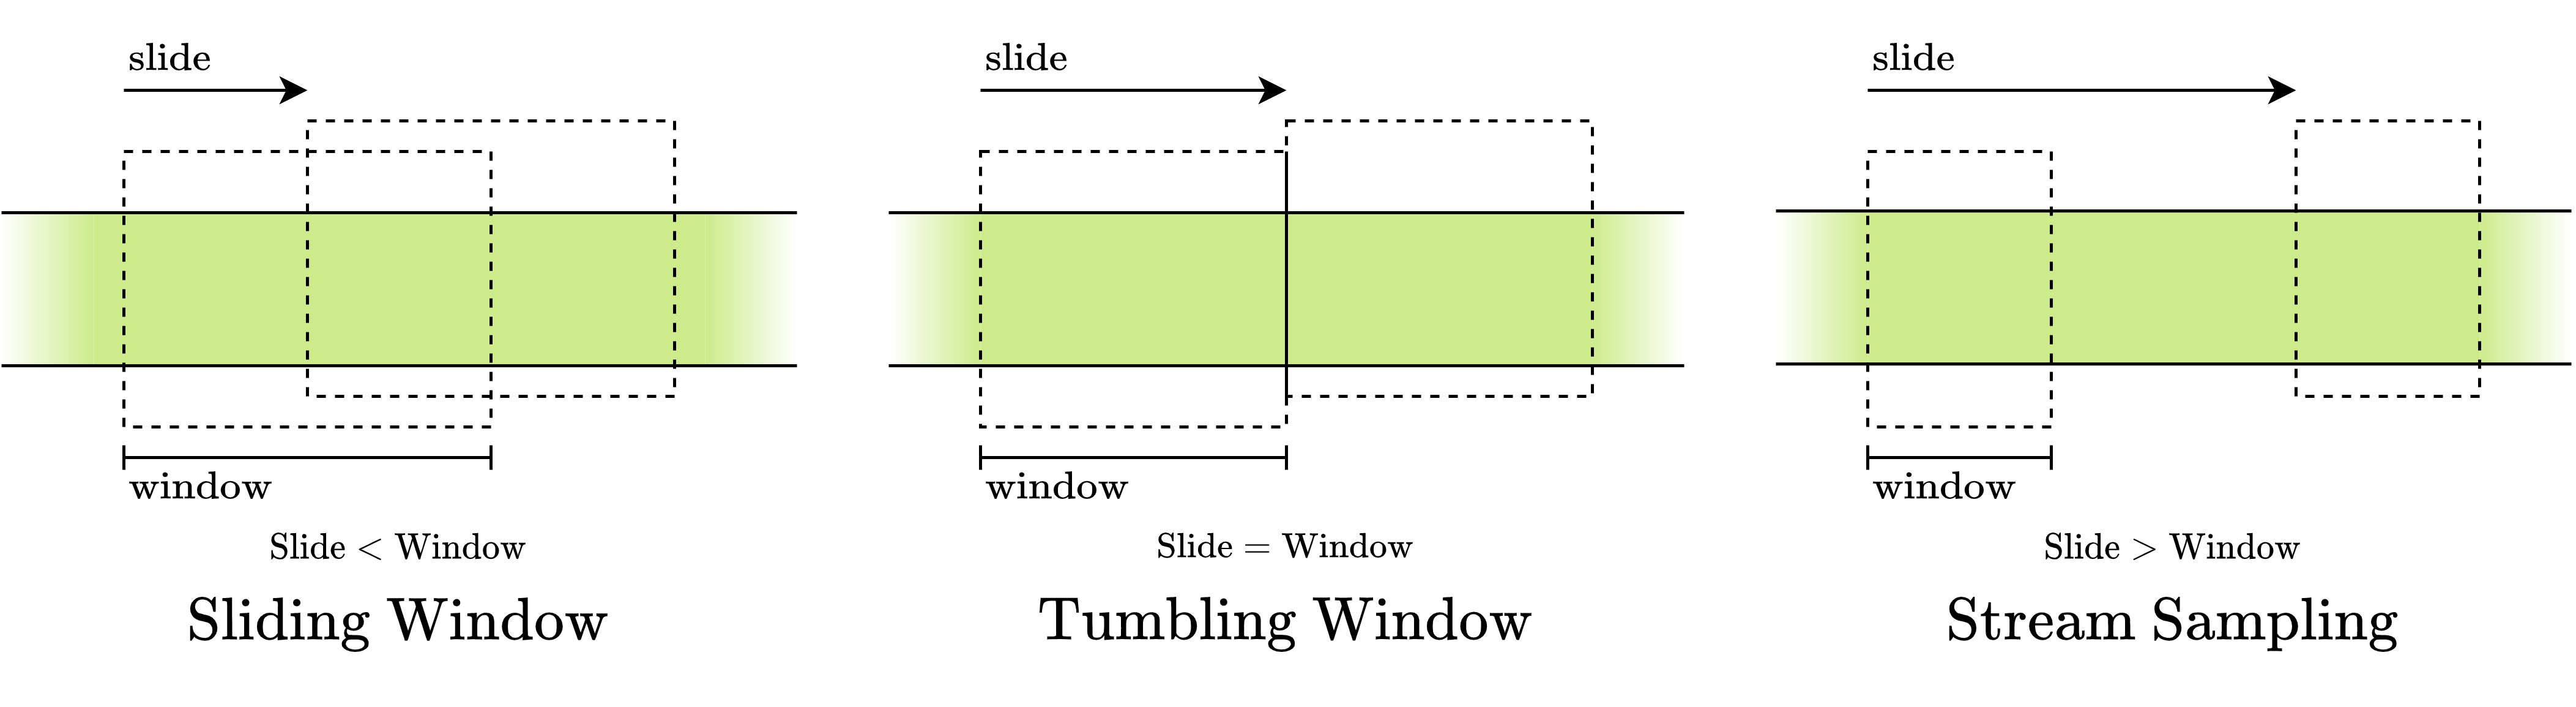
\includegraphics[width=.9\textwidth]{streams/images/window_types.drawio.png}
\end{center}
\textit{Lateness bounds} are an implementation detail for ordering streams
\\ 
\\ \textit{Windows} are SQL supported abstractions for viewing a slice of a stream, and are part of the language semantics.
\begin{sidenotebox}{SQL Windows}
    Despite being originally designed only for persistent databases, SQL added window functions in SQL 2003 (\href{https://en.wikipedia.org/wiki/SQL:2003}{see changelog}).
\end{sidenotebox}
\begin{minted}{sql}
SELECT avg(temp) OVER (
    ORDER BY timestamp
    ROWS BETWEEN 5 PRECEDING AND 5 FOLLOWING
) AS smoothed_temp
FROM SpaceStationTemp;
\end{minted}
We can run aggregate functions on a window:
\begin{minted}{sql}
min, max, sum, count -- Distributive
avg                  -- Algebraic
percentile_cont      -- Holistic
\end{minted}
Percentiles require the entire window to be read (cannot subdivide the window and combine as with \mintinline{sql}{sum}, \mintinline{sql}{count}).
\begin{definitionbox}{Invertible Function}
    \begin{center}
        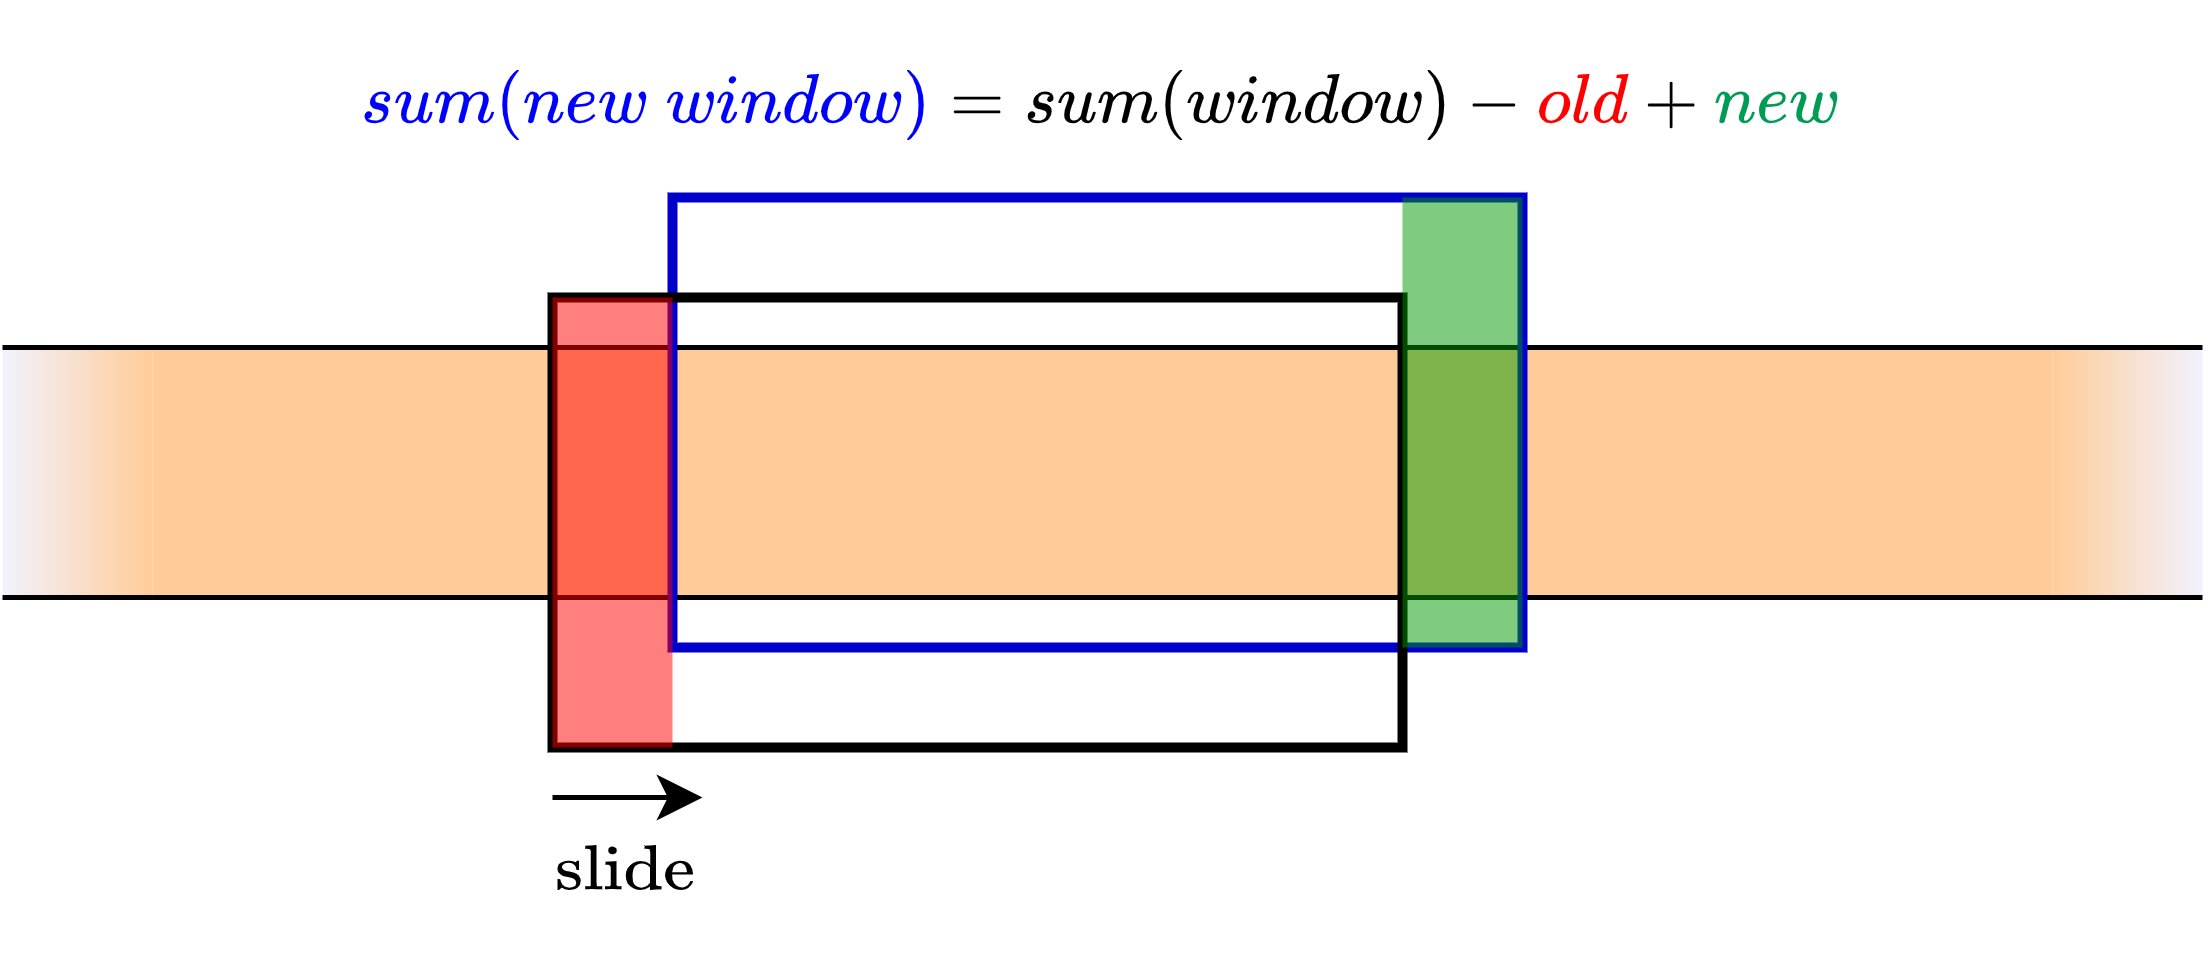
\includegraphics[width=.7\textwidth]{streams/images/invertible_agreggate.drawio.png}
    \end{center}
    Functions with an inverse that can be used to remove rows sliding out of the window from the aggregation.
    \begin{minted}{sql}
sum, count, avg       -- invertible
min, max, percentiles -- non-invertible
    \end{minted}
\end{definitionbox}

\subsection{Two Stacks Algorithm}
\begin{center}
    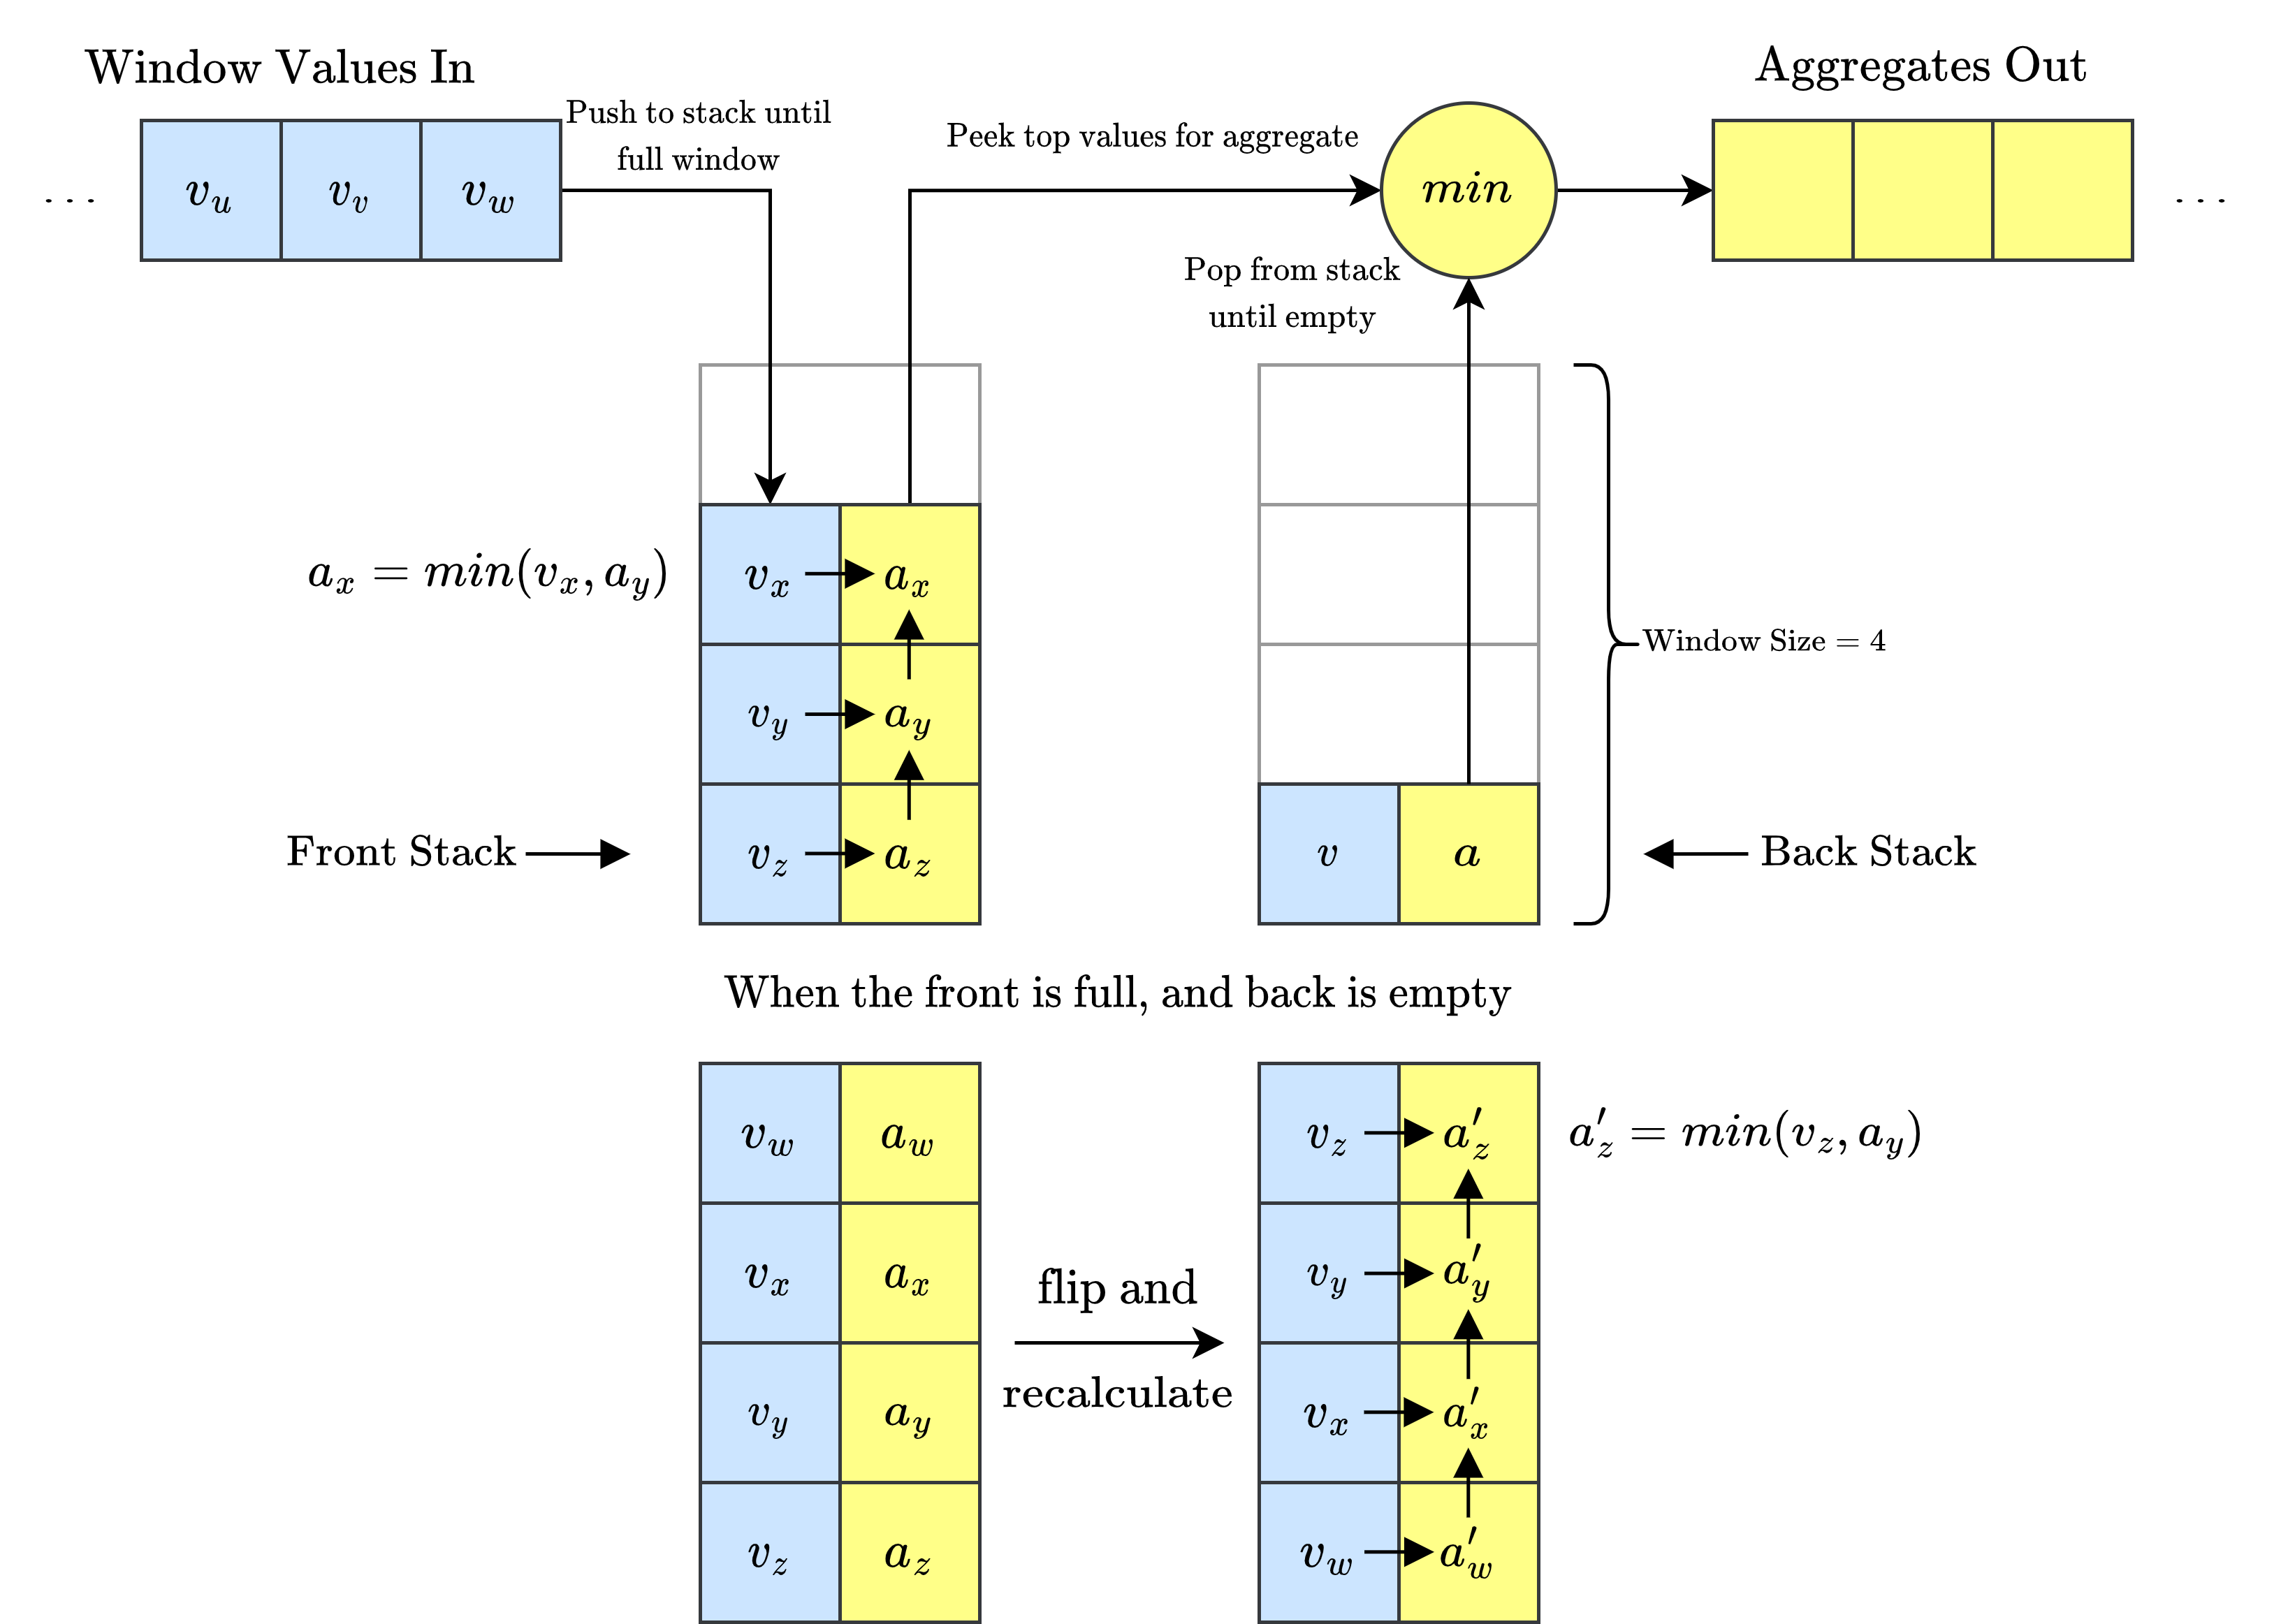
\includegraphics[width=.9\textwidth]{streams/images/two_stacks.drawio.png}
\end{center}
Two stacks of max size $window \ size$ are kept.
\begin{itemize}
    \item Each contains aggregates calculated from below adjacent aggregates and current value.
    \item When the front stack is full, and back stack empty (occurs every $\cfrac{1}{window \ size}$) flip the front stack, recalculate aggregates and set to back stack.
\end{itemize}
